% 分子平均碰壁数

\subsection{结论}

当容器中的气体平均速度为 $\bar v$, 分子数密度为 $n$ 时,单位容器面积单位时间受到分子碰撞的平均次数为
\begin{equation}
\frac14 n\bar v
\end{equation}
\subsection{推导}

假设所有分子的速度都是 $v$,分子数密度为 $n$ (单位体积内的分子数).假设分子之间不发生碰撞.如果所有的分子都向同一个方向运动,那么单位时间通过面积为 $a$ 的垂直截面的分子数为 $nva$. 如果容器是一个球壳,那么球壳的一半会受到粒子的撞击,单位时间的撞击次数(碰撞率)等于单位时间粒子通过容器最大截面的个数(如图1),即 $nv \qty(\pi R^2)$. 
\begin{figure}[ht]
\centering
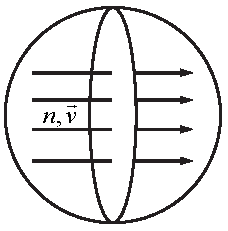
\includegraphics[width=4cm]{./figures/AvgHit1.pdf}
\caption{分子同向运动的情况} \label{AvgHit_fig1}
\end{figure}
如果有一半的分子向右移动,一半向上移动(如图2),那么每个方向的分子数密度变为原来的一半,总的碰撞率仍为
\begin{equation}
\frac12 nv \qty(\pi R^2) + \frac12 nv \qty(\pi R^2) = nv \qty(\pi R^2)
\end{equation}

\begin{figure}[ht]
\centering
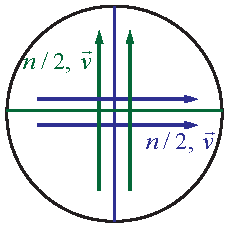
\includegraphics[width=4cm]{./figures/AvgHit2.pdf}
\caption{分子向两个方向运动的情况} \label{AvgHit_fig2}
\end{figure}
依此类推,如果分子运动的方向被均匀分布在空间的各个方向上,单位时间碰撞数仍然是.
由于球形容器的表面积为, 所以单位容器壁面积单位时间的碰撞数就是 $nv \qty(\pi R^2)$. 

接下来如果把球形容器改成任意形状的容器,由于分子运动在各个方向都是一样,所以结论不变.

另外,一般情况下并不是每个分子都具有相同的速度,所以速度取平均值 $v$ 即可.

